\documentclass{classes/exam} 
\usepackage{chemfig}
\usepackage{tikz}
\usepackage{circuitikz}
\usepackage{graphicx}
\graphicspath{{./images/}}
\usepackage[version=4]{mhchem}
%\everymath{\color{blue}}
%\pagestyle{empty}
\begin{document}
	\maketitle
	\borderline{ប្រធាន}
	\begin{enumerate}[I]
		\item {\color{magenta}\ks (១០ ពិន្ទុ)} ដូចម្តេចដែលហៅថាបម្លែងទែម៉ូឌីណាមិច? បម្លែងទែម៉ូឌីណាមិចមានប៉ុន្មានប្រភេទ?
		\\ចូរពន្យល់អំពីប្រភេទនៃបម្លែងនីមួយៗ។
		 \item {\color{magenta}\ks (១០ ពិន្ទុ)} រកប្ញសការេនៃការេល្បឿនមធ្យមរបស់ម៉ូលេគុលអុកសុីសែននៅសីតុណ្ហភាព $227^\circ C$។ \\គេឲ្យម៉ាសម៉ូលអុកសុីសែន $32\times10^{-3}kg/mol,~និង~ R=8.31J/mol\cdot K$។
		 \item {\color{magenta}\ks (១០ ពិន្ទុ)} ក្នុងរូបបង្ហាញពីវដ្តនៃឧស្ម័ន។ បម្រែបម្រួលថាមពលក្នុងនៃឧស្ម័នក្នុងលំនាំពី $a\rightarrow c$ តាមគន្លង $abc$ \\គឺ $-200J$។ ថាមពល $180J$ ត្រូវបានផ្តល់ជាកម្តៅក្នុងលំនាំពី $c\rightarrow d$។ ម្យ៉ាងទៀតថាមពល $80J$ ត្រូវបានផ្តល់ជាកម្តៅក្នុងលំនាំពី $d\rightarrow a$។ ចូរគណនាកម្មន្តដែលបំពេញដោយឧស្ម័នក្នុងលំនាំពី $c\rightarrow d$។
		 \begin{figure}[H]
		 	\centering
		 	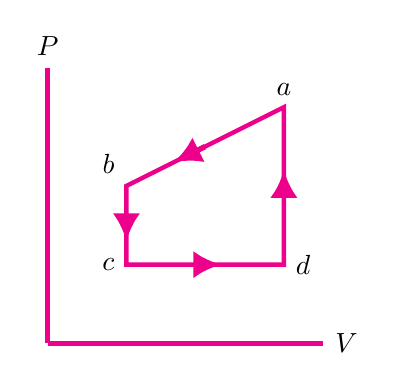
\begin{tikzpicture}[scale=1,fill=magenta, draw=magenta]
		 	\begin{scope}[line width=2pt]
		 	\draw (0,0)-- (0,3.5);
		 	\draw (0,0)-- (3.5,0);
		 	\draw [ultra thick] (1,1) -- (3,1) -- (3,3) -- (1,2) --cycle;
		 	\coordinate [label=above:$a$] (a) at (3,3);
		 	\coordinate [label=above left:$b$] (b) at (1,2);
		 	\coordinate [label=left:$c$] (c) at (1,1);
		 	\coordinate [label=right:$d$] (c) at (3,1);
		 	\coordinate [label=right:$V$] ($V$) at (3.5,0);
		 	\coordinate [label=above:$P$] ($P$) at (0,3.5);
		 	\draw [arrows = {-Latex[width=10pt, length=10pt]}] (3,2) -- (3,2.2);
		 	\draw [arrows = {-Latex[width=10pt,length=10pt]}] (2,1)--(2.2,1);
		 	\draw [arrows = {-Latex[width=10pt,length=10pt]}] (1,1.5)--(1,1.3);
		 	\draw [arrows = {-Latex[width=10pt, length=10pt]}] (2,2.5) -- (1.6,2.3);
		 	\end{scope}
		 	\end{tikzpicture}
		 \end{figure}
		\item {\color{magenta}\ks (១៥ ពិន្ទុ)} ធុងមួយមានមាឌ $V=2.5m\ell$ មានផ្ទុកឧស្ម័នដែលមានម៉ាស $50mg$ ស្ថិតក្រោមសម្ពាធ $1035kPa$។ \\ម៉ាសរបស់ម៉ូលេគុលនៃឧស្ម័ននីមួយៗគឺ $8\times10^{-26}kg$។ គេឲ្យៈ $k_{B}=1.38\times10^{-23}J/K$។
		\begin{enumerate}[k]
			\item គណនាចំនួនម៉ូលេគុលសរុបនៃឧស្ម័ននោះ។
			\item គណនាតម្លៃថាមពលសុីនេទិចមធ្យមនៃម៉ូលេគុលឧស្ម័ននីមួយៗ
			\item គណនាតម្លៃថាមពលសុីនេទិចសរុបរបស់ម៉ូលេគុលក្នុងធុង។
		\end{enumerate}
	\item {\color{magenta}\ks (១៥ ពិន្ទុ)} ក្នុងស្ថានភាពនីមួយៗដូចខាងក្រោម ចូររកបម្រែបម្រួលថាមលក្នុងនៃប្រព័ន្ធៈ
	\begin{enumerate}[k]
		\item ប្រព័ន្ធនោះទទួលកម្តៅ $500cal$ ហើយនៅពេលជាមួយគ្នានោះវាធ្វើកម្មន្ត $400J$។
		\item ប្រព័ន្ធនោះទទួលកម្តៅ $300cal$ ហើយនៅពេលជាមួយគ្នានោះកម្មន្ត $420J$ បានធ្វើមកលើប្រព័ន្ធ។
		\item កម្តៅ $1200cal$ ត្រូវបានដកចេញពីឧស្ម័ន គេឃើញមាឌថេរ។ គេឲ្យៈ $1cal=4.2J$ 
	\end{enumerate}
	\item {\color{magenta}\ks (១៥ ពិន្ទុ)} ធុងមួយមានពីរផ្នែក ដែលផ្នែកទី១ដាក់ឧស្ម័នបរិសុទ្ធមួយប្រភេទដែលមានចំនួនម៉ូល $n_{1}$ និងផ្នែកទី២ ដាក់ឧស្ម័នបរិសុទ្ធមួយប្រភេទទៀតដែលមានចំនួនម៉ូល $n_{2}$។ នៅចន្លោះឧស្ម័នទាំងពីរមានពីស្តុងដែលអាចចល័តបាន និងមានកម្រាស់អាចចោលបានដូចរូប។ ក្នុងធុងនោះមានឧស្ម័នសរុបចំនួន $20$ ម៉ូល។ នៅពេលដែលប្រព័ន្ធមានសីតុណ្ហភាព និងសម្ពាធដូចគ្នា ប្រវែង $\ell_{1}=90cm$ និង $\ell_{2}=30cm$។ គណនា ចំនួនម៉ូល $n_{1}$ និង $n_{2}$។
		\begin{figure}[H]
			\centering
			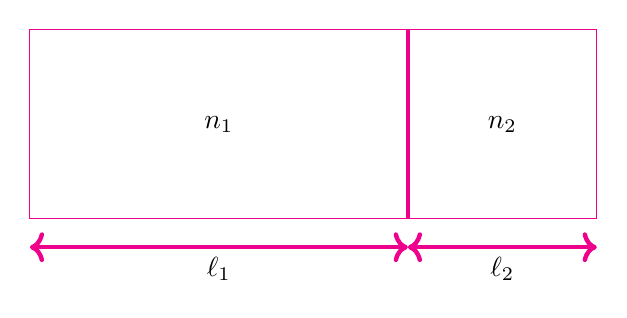
\begin{tikzpicture}[fill=magenta, draw=magenta, scale=1.2]
			\begin{scope}]
			\coordinate (A) at (0,0);
			\coordinate (B) at (6,0);
			\coordinate (C) at (6,2);
			\coordinate (D) at (0,2);
			\coordinate[label=below:{$\ell_{1}$}] (L1) at (2,-.3);
			\coordinate[label=below:{$\ell_{2}$}] (L1) at (5,-.3);
			\draw (A)--(B)--(C)--(D)--cycle;
			\draw[ultra thick] (4,0)--(4,2);
			\node at (2,1) {$n_{1}$};
			\node at (5,1) {$n_{2}$};
			\draw[<->, ultra thick] (0,-.3)--(4,-.3);
			\draw[<->, ultra thick] (4,-.3)--(6,-.3);
			\end{scope}
			\end{tikzpicture}
		\end{figure}
	\end{enumerate}
%%%%%%%%%%%%%%%%%%%% អត្រាកំណែ %%%%%%%%%%%%%%%%%%%%%%%%%%
\newpage
\borderline{អត្រាកំណែ}
\begin{enumerate}[I]
	\item {\color{magenta}\ks (១០ ពិន្ទុ)} បម្លែងទែម៉ូឌីណាមិចៈ ប្រព័ន្ធមួយទទួលបម្លែងទែម៉ូឌីណាមិច កាលណាវាផ្លាស់ប្តូរភាព ដោយប្តូរតែ កម្មន្ត និងកម្តៅ ជាមួយមជ្ឈដ្ឋានក្រៅប៉ុណ្ណោះ។ គេចែកបម្លែងទែម៉ូឌីណាមិចជាពីរគឺ បម្លែងចំហ និងបម្លែងបិទ។
	\begin{itemize}
		\item បើភាពដើម និងភាពស្រេចនៃប្រព័ន្ធមួយ ខុសគ្នា នោះគេថាប្រព័ន្ធទទួលរងនូវបម្លែចំហ។
		\item បើភាពដើម និងភាពស្រេចនៃប្រព័ន្ធមួយ ដូចគ្នា នោះគេថាប្រព័ន្ធទទួលរងនូវបម្លែងបិទ។
	\end{itemize}
	\item {\color{magenta}\ks (១០ ពិន្ទុ)} រកប្ញសការេនៃការេល្បឿនមធ្យមរបស់ម៉ូលេគុលអុកសុីសែន
	\begin{flalign*}
		\text{តាម}\quad :&\quad \upsilon_{rms}=\sqrt{\frac{3RT}{M_{\ce{O2}}}}\\
		\text{ដោយ}\quad :&\quad M_{\ce{O2}}=32\times10^{-3}kg/mol,~R=8.31J/mol\cdot K\\
		\quad :&\quad T=227+273=500K\\
		\text{គេបាន}\quad :&\quad \upsilon_{rms}=\sqrt{\frac{3\times8.31\times500}{32\times10^{-3}}}=\sqrt{389531}=624.124m/s\\
		\text{ដូចនេះ}\quad :&\quad \upsilon_{rms}=624.124m/s
	\end{flalign*}
	\item {\color{magenta}\ks (១០ ពិន្ទុ)} គណនាកម្មន្តដែលបំពេញដោយឧស្ម័នក្នុងលំនាំពី $c\rightarrow d$
	\begin{figure}[H]
		\centering
		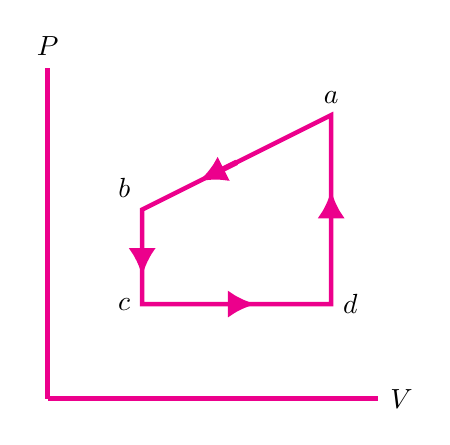
\begin{tikzpicture}[scale=1.2,fill=magenta, draw=magenta]
		\begin{scope}[line width=2pt]
		\draw (0,0)-- (0,3.5);
		\draw (0,0)-- (3.5,0);
		\draw [ultra thick] (1,1) -- (3,1) -- (3,3) -- (1,2) --cycle;
		\coordinate [label=above:$a$] (a) at (3,3);
		\coordinate [label=above left:$b$] (b) at (1,2);
		\coordinate [label=left:$c$] (c) at (1,1);
		\coordinate [label=right:$d$] (c) at (3,1);
		\coordinate [label=right:$V$] ($V$) at (3.5,0);
		\coordinate [label=above:$P$] ($P$) at (0,3.5);
		\draw [arrows = {-Latex[width=10pt, length=10pt]}] (3,2) -- (3,2.2);
		\draw [arrows = {-Latex[width=10pt,length=10pt]}] (2,1)--(2.2,1);
		\draw [arrows = {-Latex[width=10pt,length=10pt]}] (1,1.5)--(1,1.3);
		\draw [arrows = {-Latex[width=10pt, length=10pt]}] (2,2.5) -- (1.6,2.3);
		\end{scope}
		\end{tikzpicture}
	\end{figure}
	\begin{flalign*}
		\text{តាម}\quad :&\quad Q_{cd}=W_{cd}+\Delta U_{cd}~\Rightarrow~W_{cd}=Q_{cd}-\Delta U_{cd}\\
		\text{យើងមាន}\quad :&\quad \Delta U_{ac}=-200J,~Q_{cd}=180J,~Q_{da}=80J\\
		\quad :&\quad W_{da}=0~(\text{លំនាំអុីសូករ})~\text{នោះ}~\Delta U_{da}=Q_{da}=80J\\
		\text{ម្យ៉ាងទៀត}\quad :&\quad \Delta U=0~(\text{បម្លែងបិទ})\\
		\quad :&\quad \Delta U_{ac}+\Delta U_{cd}+\Delta U_{da}=0\\
		\text{នាំឲ្យ}\quad :&\quad \Delta U_{cd}=-\Delta U_{ac}-\Delta U_{da}=-\left(-200\right)-80=120J\\
		\text{គេបាន}\quad :&\quad W_{cd}=180-120=60J\\
		\text{ដូចនេះ}\quad :&\quad W_{cd}=60J
	\end{flalign*}
	\newpage
	\item {\color{magenta}\ks (១៥ ពិន្ទុ)}
	\begin{enumerate}[k]
		\item គណនាចំនួនម៉ូលេគុលសរុបនៃឧស្ម័ននោះ។
		\begin{flalign*}
			\text{តាម}\quad :&\quad m=m_{0}N~\Rightarrow~N=\frac{m}{m_{0}}\\
			\text{ដោយ}\quad :&\quad m=50mg=50\times10^{-6}kg,~m_{0}=8\times10^{-26}kg\\
			\text{គេបាន}\quad :&\quad N=\frac{50\times10^{-6}}{8\times10^{-26}}=6.25\times10^{20}~\text{ម៉ូលេគុល}\\
			\text{ដូចនេះ}\quad :&\quad N=6.25\times10^{20}~\text{ម៉ូលេគុល}
		\end{flalign*}
		\item គណនាតម្លៃថាមពលសុីនេទិចមធ្យមនៃម៉ូលេគុលឧស្ម័ននីមួយៗ
			\begin{flalign*}
				\text{តាម}\quad :&\quad K_{av}=\frac{3}{2}k_{B}T\\
				\text{តែ}\quad :&\quad PV=Nk_{B}T~\Rightarrow k_{B}T=\frac{PV}{N}\\
				\text{នោះ}\quad :&\quad K_{av}=\frac{3}{2}\frac{PV}{N}\\
				\text{ដោយ}\quad :&\quad N=6.25\times10^{20}~\text{ម៉ូលេគុល},~P=1035kPa=1035\times10^{3}Pa\\
				\quad :&\quad V=2.5m\ell=2.5\times10^{-6}m^{3}\\
				\text{គេបាន}\quad :&\quad K_{av}=\frac{3}{2}\times\frac{1035\times10^{3}\times2.5\times10^{-6}}{6.25\times10^{20}}=62.1\times10^{-22}J\\
				\text{ដូចនេះ}\quad :&\quad K_{av}=62.1\times10^{-22}J
			\end{flalign*}
		\item គណនាតម្លៃថាមពលសុីនេទិចសរុបរបស់ម៉ូលេគុលក្នុងធុង។
		\begin{flalign*}
			\text{តាម}\quad :&\quad K=NK_{av}\\
			\text{ដោយ}\quad :&\quad N=6.25\times10^{20}~\text{ម៉ូលេគុល},~K_{av}=62.1\times10^{-22}J\\
			\text{គេបាន}\quad :&\quad K=6.25\times10^{20}\times62.1\times10^{-22}=388.125\times10^{-2}J\\
			\text{ដូចនេះ}\quad :&\quad K=388.125\times10^{-2}J
		\end{flalign*}
	\end{enumerate}
	\item {\color{magenta}\ks (១៥ ពិន្ទុ)} រកបម្រែបម្រួលថាមលក្នុងនៃប្រព័ន្ធៈ
	\begin{flalign*}
		\text{តាម}\quad :&\quad Q=W+\Delta U~\Rightarrow~\Delta U=Q-W
	\end{flalign*}
	
	\begin{enumerate}[k]
		\item ប្រព័ន្ធនោះទទួលកម្តៅ $500cal$ ហើយនៅពេលជាមួយគ្នានោះវាធ្វើកម្មន្ត $400J$។
		\begin{flalign*}
			\text{ដោយ}\quad :&\quad Q=500cal=500\times4.2=2100J,~W=400J\\
			\text{គេបាន}\quad :&\quad \Delta U=2100-400=1700J\\
			\text{ដូចនេះ}\quad :&\quad \Delta U=1700J
		\end{flalign*}
		\item ប្រព័ន្ធនោះទទួលកម្តៅ $300cal$ ហើយនៅពេលជាមួយគ្នានោះកម្មន្ត $420J$ បានធ្វើមកលើប្រព័ន្ធ។
		\begin{flalign*}
			\text{ដោយ}\quad :&\quad Q=300cal=300\times4.2=1260J,~W=-420J~(\text{កម្មន្តធ្វើលើប្រព័ន្ធ})\\
			\text{គេបាន}\quad :&\quad \Delta U=1260-\left(-420\right)=1680J\\
			\text{ដូចនេះ}\quad :&\quad \Delta U=1680J
		\end{flalign*}
		\item កម្តៅ $1200cal$ ត្រូវបានដកចេញពីឧស្ម័ន គេឃើញមាឌថេរ។
		\begin{flalign*}
			\text{ដោយ}\quad :&\quad Q=-1200cal=-1200\times4.2=-5040J,~W=0J~(\text{មាឌនៃប្រព័ន្ធមានតម្លៃថេរ})\\
			\text{គេបាន}\quad :&\quad \Delta U=-5040-0=-5040J\\
			\text{ដូចនេះ}\quad :&\quad \Delta U=-5040J
		\end{flalign*}
	\end{enumerate}
	\item {\color{magenta}\ks (១៥ ពិន្ទុ)} គណនា ចំនួនម៉ូល $n_{1}$ និង $n_{2}$
	\begin{figure}[H]
		\centering
		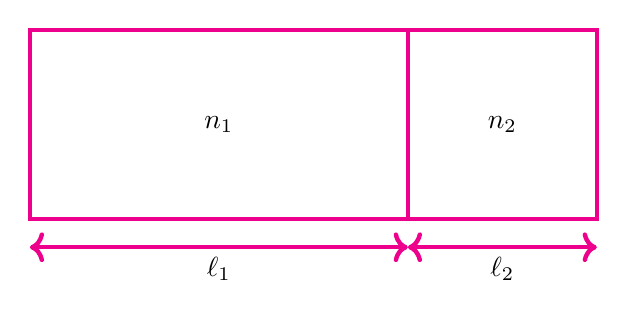
\begin{tikzpicture}[fill=magenta, draw=magenta, scale=1.2]
			\coordinate (A) at (0,0);
			\coordinate (B) at (6,0);
			\coordinate (C) at (6,2);
			\coordinate (D) at (0,2);
			\coordinate[label=below:{$\ell_{1}$}] (L1) at (2,-.3);
			\coordinate[label=below:{$\ell_{2}$}] (L1) at (5,-.3);
			\draw[ultra thick] (A)--(B)--(C)--(D)--cycle;
			\draw[ultra thick] (4,0)--(4,2);
			\node at (2,1) {$n_{1}$};
			\node at (5,1) {$n_{2}$};
			\draw[<->, ultra thick] (0,-.3)--(4,-.3);
			\draw[<->, ultra thick] (4,-.3)--(6,-.3);
		\end{tikzpicture}
	\end{figure}
	\begin{flalign*}
		\text{យើងមាន}\quad :&\quad n_{1}+n_{2}=20mol,~V_{1}=A\ell_{1},~\text{និង}~V_{2}=A\ell_{2}\\
		\quad :&\quad P_{1}=P_{2}~ \text{និង}~T_{1}=T_{2}\\
		\text{ផ្នែកទី១}\quad :&\quad P_{1}V_{1}=n_{1}RT_{1}~\Rightarrow~n_{1}=\frac{P_{1}V_{1}}{RT_{1}}\\
		\text{ផ្នែកទី២}\quad :&\quad P_{2}V_{2}=n_{2}RT_{2}~\Rightarrow~n_{2}=\frac{P_{2}V_{2}}{RT_{2}}\\
		\text{តាមផលធៀប}\quad :&\quad \dfrac{n_{1}}{n_{2}}=\dfrac{\frac{P_{1}V_{1}}{RT_{1}}}{\frac{P_{2}V_{2}}{RT_{2}}}=\frac{V_{1}}{V_{2}}=\frac{A\ell_{1}}{A\ell_{2}}=\frac{\ell_{1}}{\ell_{2}}\\
		\text{នាំឲ្យ}\quad :&\quad n_{1}=\frac{\ell_{1}}{\ell_{2}}n_{2}~\left(\ell_{1}=90cm,~\ell_{2}=30cm\right)\\
		\quad :&\quad n_{1}=\frac{90}{30}n_{2}=3n_{2}\\
		\text{គេបាន}\quad :&\quad 3n_{2}+n_{2}=20~\Rightarrow~n_{2}=\frac{20}{4}=5mol\\
		\quad :&\quad n_{1}=3\times5=15mol\\
		\text{ដូចនេះ}\quad :&\quad n_{1}=15mol~\text{និង}~n_{2}=5mol
	\end{flalign*}
\end{enumerate}
\end{document}